\documentclass[12pt,letterpaper]{article}
\usepackage[moduleName={Spectre},version={2.1.2}]{ArhythmeticUnits}

\begin{document}
\titlePage{img/Logo}{img/Module}{img/ArhythmeticUnits}{}

% ----------------------------------------------------------------------------
% MARK: Overview
% ----------------------------------------------------------------------------

\section{Overview}

\textbf{Spectre} is a spectrogram visualizer for VCV Rack 2. It shows how a
signal's frequency content changes over time: frequency runs from bottom to
top, successive spectra occupy columns across the display, and color
represents magnitude. Spectre has one signal input and no audio outputs.
Patch it alongside your audio path to inspect a signal without changing what
you hear.

Fourier and Spectre belong to the Arhythmetic Units Fourier plugin. Use
Fourier to compare the current spectra of up to four signals, and Spectre to
follow one signal's spectrum over time. Both provide the same window choices
and smoothing controls, but their display axes, input-gain defaults, and Run
behavior differ as described below.

Spectre uses a short-time Fourier transform (STFT) with a fixed FFT length of
2048 samples, a hop size of 1024 samples (50\% overlap), and a history of 512
spectra. FFT length, hop size, and history length are not adjustable. You can
choose the window function, time and frequency smoothing, visible frequency
range, display slope, and color map.

At sample rate $f_s$, frequency bins are spaced $f_s/2048$ Hz apart, each
analysis window spans $2048/f_s$ seconds, and a complete display sweep takes
$512 \times 1024/f_s$ seconds. At $48\,\mathrm{kHz}$, these are approximately
$23.4\,\mathrm{Hz}$, $42.7\,\mathrm{ms}$, and $10.92\,\mathrm{s}$
respectively. At $44.1\,\mathrm{kHz}$, a sweep takes about
$11.89\,\mathrm{s}$. Increasing Rack's sample rate shortens the history
duration and increases the spacing between bins.

\clearpage
\section{Quick Start}

\begin{itemize}
  \item Connect an oscillator or another signal to the input. The illuminated
  \textbf{Run} button indicates that Spectre is acquiring new spectra.
  Keep your existing connection to the mixer or audio output if you want to
hear it.
  \item A new module uses $+6\,\mathrm{dB}$ input gain, a Flattop window,
  and no time or frequency smoothing. For comparisons with Fourier, set
  both modules to the same input gain; Fourier starts at $0\,\mathrm{dB}$.
  \item A steady sine wave produces a horizontal band. Harmonics appear as
  additional bands above it; short broadband sounds produce vertical marks.
  \item Adjust the input gain if the image is too faint or too much of it
  reaches the color map's brightest end. Set \textbf{Slope} to zero when you
  want to compare magnitudes without frequency-dependent display weighting.
  The default is $+4.5\,\mathrm{dB/oct}$.
  \item Press \textbf{Run} to freeze the history, then hover over the plot to
  inspect a frequency and its magnitude. Press it again to resume.
\end{itemize}

\paragraph{Reading levels} Spectre displays spectral magnitudes, not total
signal RMS, loudness, or sound pressure level. Window choice, frequency
alignment with FFT bins, and smoothing affect the height and width of a peak.
The color map has a finite range; reaching its end color does not mean Spectre
has clipped your audio path. The hover readout measures stored magnitudes
before Slope weighting.

\paragraph{Choosing settings} Use little or no \textbf{Average} to follow
changes more closely. Increase \textbf{Average} for a steadier image and
\textbf{Smooth} for a broader view of tonal balance. FFT length and hop size
are fixed; cropping the frequency range enlarges existing detail without
increasing resolution. The factory presets provide examples of these choices.

% ----------------------------------------------------------------------------
% MARK: Panel Layout
% ----------------------------------------------------------------------------

\clearpage
\section{Panel Layout}

\begin{figure}[!htp]
\centering
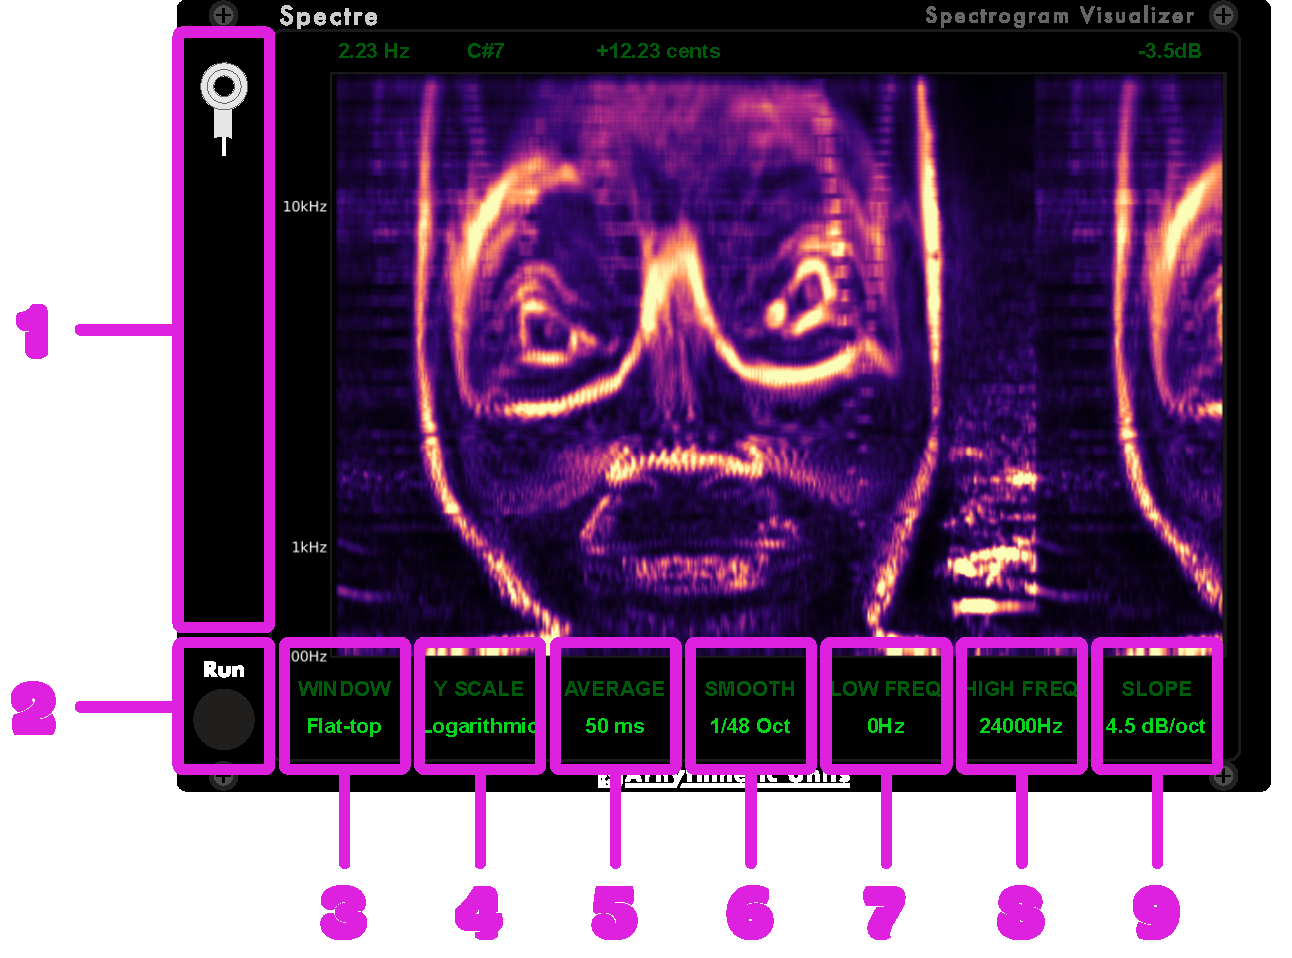
\includegraphics[width=\textwidth]{img/PanelLayout}
\caption{Spectre's input, Run button, and display controls.}
\end{figure}

The numbered illustration identifies control positions. The sections below
give the current ranges and defaults.

\subsection{Input}

The single \textbf{Input} accepts monophonic or polyphonic cables. \textbf{All
voices on the port are summed into one analyzed signal}; voices are not drawn
separately. Summed voices can increase the level or cancel one another,
depending on their phase. The input is normalized so that $\pm5\,\mathrm{V}$
corresponds to $\pm1$ before gain.

\textbf{Input Gain} ranges from silence ($-\infty\,\mathrm{dB}$) to
$+12\,\mathrm{dB}$ and starts at $+6\,\mathrm{dB}$. It changes the signal
being analyzed, not the gain of your audio path. Lower it if strong signals or
summed voices saturate the color map. Gain changes affect newly acquired
spectra; they do not rescale the stored history.

\subsection{Run}

When \textbf{Run} is lit, Spectre buffers and analyzes incoming samples. When
it is dark, buffering and FFT processing pause and the current history remains
available for inspection. Resuming continues from the paused position; audio
received during the pause is not captured. Run is initially enabled.

While frozen, you can change \textbf{Y Scale}, \textbf{LO Freq}, \textbf{HI
Freq}, \textbf{Slope}, and the \textbf{Color Map} to view the same history
differently. Input gain, window, \textbf{Average}, \textbf{Smooth}, and
AC-coupling changes affect subsequent analysis after you resume, not spectra
already in the history.

\subsection{Window Function}

The \textbf{Window} control selects the function applied to each audio frame
before the FFT. Windowing changes the balance between peak width and
\textit{spectral leakage}, the spreading of a tone into nearby bins when its
frequency does not fit the analysis frame exactly.

The 15 choices are Boxcar, Bartlett, BartlettHann, Parzen, Welch, Cosine,
Bohman, Lanczos, Hann, Hamming, Blackman, BlackmanHarris, BlackmanNuttall,
KaiserBessel, and Flattop. \textbf{Flattop} is the default. These are fixed
window shapes; the control selects a shape without additional shape
parameters.

Boxcar leaves the samples untapered and has a narrow main peak but strong
leakage for tones between bins. Hamming reduces leakage at the cost of a wider
peak. Flattop has a broader peak and is useful for comparing tone amplitudes
as the tone moves between bins. Spectre compensates for the window's coherent
gain, but different windows still produce different peak shapes and noise
levels.

Changing the window affects new spectra; it does not recalculate the history.

\subsection{Y Scale}

\textbf{Y Scale} offers \textbf{Linear} and \textbf{Logarithmic} (the
default). Linear places equal frequency intervals at equal distances. The mode
named Logarithmic expands the low-frequency portion of the view. In this
version, it uses a square-root mapping of frequency, so equal octaves are not
equally spaced. Read the axis labels or cursor frequency rather than treating
it as a mathematically logarithmic axis. Frequency is on Spectre's vertical
axis; Fourier uses \textbf{X Scale} for frequency and \textbf{Y Scale} for
amplitude.

\subsection{Average}

\textbf{Average} controls exponential smoothing of spectral magnitudes over
time, from $0$ to $2500\,\mathrm{ms}$; the default is
\textbf{$0\,\mathrm{ms}$} (off). Higher values produce a steadier display that
reacts more slowly. This is a recursive filter, not an arithmetic average over
a fixed recording of the selected duration.

In Spectre, smoothing can blur transients across time; its duration is not the
length of the visible history.

\clearpage
\subsection{Smooth}

\textbf{Smooth} combines neighboring spectral magnitudes over a
fractional-octave band. Its default is \textbf{None}. Available widths are
$1/48$, $1/24$, $1/12$, $1/9$, $1/6$, $1/5$, $1/4$, $1/3$, $1/2$, $2/3$,
$3/4$, 1, 1.5, 2, and 2.5 octaves. Wider settings hide more fine detail and
can lower narrow peaks. Use None when inspecting individual harmonics.
Smoothing does not improve the FFT's frequency resolution.

\subsection{Low Frequency}

\textbf{LO Freq} sets the bottom of the displayed frequency range, in Hz. It
defaults to $0\,\mathrm{Hz}$ and can be set up to half the sample rate (the
Nyquist frequency). This control crops the view; it does not filter the input
or remove frequencies from the stored analysis.

\subsection{High Frequency}

\textbf{HI Freq} sets the top of the displayed frequency range, in Hz. It
defaults to the Nyquist frequency, which is also its maximum. At
$48\,\mathrm{kHz}$, this is $24\,\mathrm{kHz}$. Keep LO Freq strictly below HI
Freq for a usable display. Zooming into a smaller frequency range enlarges the
existing bins without adding frequency detail.

\subsection{Slope}

\textbf{Slope} applies frequency-dependent weighting when coloring the image.
Its range is $-9$ to $+9\,\mathrm{dB/oct}$, with a default of
$+4.5\,\mathrm{dB/oct}$. Positive values emphasize the upper part of the
display, negative values emphasize the lower part, and zero disables this
weighting. It can be changed while frozen and does not alter the stored
magnitudes or the hover dB readout.

The weighting is referenced to $1\,\mathrm{kHz}$ on the Linear scale. In
Logarithmic mode it is applied using the image-row position before the
frequency mapping, so it is not an exact dB-per-octave correction at the
labeled frequencies. Use zero slope for unweighted comparisons.

% ----------------------------------------------------------------------------
% MARK: Display And Settings
% ----------------------------------------------------------------------------

\clearpage
\section{Reading The Display}

The scan line advances from left to right and wraps back to the left edge.
Each new column replaces the oldest spectrum at that position. The image
does not scroll: the newest spectrum is immediately behind the scan line
(to its left, except at the wrap), and older history lies ahead of it.
A frozen history excludes any elapsed time while Run was off.

Color represents linear magnitude after gain, windowing, smoothing, and
Slope weighting. The color map has a finite range: magnitudes above its
upper limit share the same end color. A bright region therefore does not
show how far above that limit the signal is. Lower the input gain and
acquire new history to distinguish those levels.

Hover over the plot for a crosshair and readouts of frequency, musical note,
tuning offset, and magnitude in dB. The magnitude comes from the stored
spectrum at that time and frequency, before Slope weighting. Unlike Fourier's
amplitude readout, which describes the cursor position, Spectre's readout
measures a stored spectral bin. The display has no time readout; use the sweep
duration described in the overview as a guide.

\section{Context Menu And Saved Settings}

Right-click the module to find these options under \textbf{Render Settings}:
\begin{itemize}
  \item \textbf{AC-coupled} removes DC offset from newly captured inputs
  using a DC-blocking filter. It is on by default and can also affect very
  low frequencies. Turn it off when inspecting DC or slow signals, and set
  Slope to zero to avoid frequency weighting near DC. This setting does not
  reprocess history.
  \item \textbf{Color Map}: Viridis, Cividis, Magma, Plasma, Inferno, Bone,
  or Gray. Magma is the default. Selecting another map recolors the existing
  history, including while frozen.
\end{itemize}

These menu changes support Rack's Undo and Redo commands. Patches and module
presets save the panel settings, Run state, AC-coupling choice, and color map.
They do not save the recorded spectrogram. A patch saved while frozen reopens
with no recorded history; enable Run to acquire a new image.

Rack's module initialization resets the controls to their defaults, enables
Run and AC coupling, selects Magma, and clears the history. Changing Rack's
sample rate changes the available frequency range, bin spacing, and sweep
duration. Existing history is not cleared automatically and is displayed
using the new frequency mapping; allow a full sweep to replace it before
comparing frequencies at the new sample rate.

\clearpage
\section{Factory Presets}

Load these examples from Rack's module preset menu. All start running, with
$0\,\mathrm{dB}$ input gain and the Magma color map. Frequency bounds are
limited by the current sample rate. Unlike Fourier's presets, these cannot
change FFT length or hop size; both remain fixed in Spectre.

\begin{description}[style=nextline, leftmargin=0pt, labelwidth=0pt, labelsep=0pt]
  \item[Mastering] Broad tonal balance: Flattop, Logarithmic Y Scale,
  $0$--$20\,\mathrm{kHz}$, Average $300\,\mathrm{ms}$, Smooth $1/12$ octave,
  Slope $+4.5\,\mathrm{dB/oct}$. AC coupling is on.
  \item[Harmonics] Individual harmonics: Hann, Linear Y Scale,
  $0$--$5\,\mathrm{kHz}$. Average and Smooth are off; Slope is zero.
  AC coupling is on.
  \item[BassDetail] Low-frequency view: Hann, Linear Y Scale,
  $0$--$500\,\mathrm{Hz}$, Average $100\,\mathrm{ms}$. Smooth is off and
  Slope is zero. AC coupling is on. Cropping the view does not provide the
  finer bin spacing of Fourier's longer FFT in its BassDetail preset.
  \item[Transients] Unsmoothed changes over time: Hann, Logarithmic Y Scale,
  $0$--$20\,\mathrm{kHz}$. Average and Smooth are off; Slope is zero.
  AC coupling is on. Frame duration and update interval remain fixed.
  \item[PluginDevelopment] Unweighted spectrum including DC: Flattop,
  Linear Y Scale, $0$--$20\,\mathrm{kHz}$. Average and Smooth are off;
  Slope is zero. AC coupling is off.
\end{description}

\clearpage
\section{Troubleshooting}

\begin{description}[style=nextline, leftmargin=0pt, labelwidth=0pt, labelsep=0pt]
  \item[No image or a stale image] Check the source signal, cable, input
  gain, and Run light. Ensure LO Freq is below HI Freq. If you loaded a
  frozen patch, resume capture to acquire new history.
  \item[Bands are too broad or changes blur together] Reduce Smooth and
  Average, and compare window functions. Spectre's FFT length is fixed;
  use Fourier if you need a longer frame to separate nearby frequencies.
  \item[Levels differ from another analyzer] Match input gain, window,
  FFT length, smoothing, and amplitude reference. Set Slope to zero and
  account for summed polyphonic voices. Spectre starts at $+6\,\mathrm{dB}$
  input gain; Fourier starts at $0\,\mathrm{dB}$. A spectral peak is not a
  broadband RMS measurement.
  \item[Large regions reach the same end color] Reduce input gain and
  acquire new history. Saturated colors cannot show how far a magnitude
  exceeds the color map's range. Recoloring alone cannot recover that
  distinction in the displayed image.
  \item[Old and new bands disagree after a sample-rate change] Allow a full
  sweep to replace history acquired at the old sample rate before comparing
  frequencies. Check the frequency bounds as well.
  \item[Analysis uses too much CPU] Spectre performs analysis on Rack's
  audio engine thread despite having no audio outputs. Turn Run off when
  inspecting a frozen image to pause buffering and FFT processing. Its FFT
  length and hop size are fixed; Fourier provides adjustable settings when
  you need to trade frequency detail or update rate for analysis workload.
\end{description}

\section{Analysis Timing And Further Reading}

Spectre prepares each new spectrum over its 1024-sample update interval,
about $21.3\,\mathrm{ms}$ at $48\,\mathrm{kHz}$. Each spectrum already covers
about $42.7\,\mathrm{ms}$ of audio at that rate. Average and Rack's display
refresh add further visible delay.

Analysis settings take effect at the start of the next frame and affect new
columns. Turning Run off pauses any unfinished frame; resuming completes it
before starting another. Changing Rack's sample rate discards unfinished
analysis. Allow new history to replace older columns before comparing results
across that change.

Analysis runs on Rack's audio engine thread. Work is spread across sample
calls to reduce processing bursts, but the module still contributes to the
patch's CPU load. This does not guarantee that a heavily loaded patch will
meet its audio deadlines.

For the mathematical background, FFT algorithms, scheduling proofs, and
performance experiments, see the accompanying
\href{https://github.com/Kautenja/ArhythmeticUnits-Fourier/tree/main/docs/whitepaper}{\textit{Fourier technical report}}.
Its implementation appendix gives the supporting algorithms; this manual
focuses on operating the module.

% ----------------------------------------------------------------------------
% MARK: Copyright seal
% ----------------------------------------------------------------------------

\clearpage
\finalPage

\end{document}
